\documentclass{article}\usepackage[]{graphicx}\usepackage[]{color}
%% maxwidth is the original width if it is less than linewidth
%% otherwise use linewidth (to make sure the graphics do not exceed the margin)
\makeatletter
\def\maxwidth{ %
  \ifdim\Gin@nat@width>\linewidth
    \linewidth
  \else
    \Gin@nat@width
  \fi
}
\makeatother

\definecolor{fgcolor}{rgb}{0.345, 0.345, 0.345}
\newcommand{\hlnum}[1]{\textcolor[rgb]{0.686,0.059,0.569}{#1}}%
\newcommand{\hlstr}[1]{\textcolor[rgb]{0.192,0.494,0.8}{#1}}%
\newcommand{\hlcom}[1]{\textcolor[rgb]{0.678,0.584,0.686}{\textit{#1}}}%
\newcommand{\hlopt}[1]{\textcolor[rgb]{0,0,0}{#1}}%
\newcommand{\hlstd}[1]{\textcolor[rgb]{0.345,0.345,0.345}{#1}}%
\newcommand{\hlkwa}[1]{\textcolor[rgb]{0.161,0.373,0.58}{\textbf{#1}}}%
\newcommand{\hlkwb}[1]{\textcolor[rgb]{0.69,0.353,0.396}{#1}}%
\newcommand{\hlkwc}[1]{\textcolor[rgb]{0.333,0.667,0.333}{#1}}%
\newcommand{\hlkwd}[1]{\textcolor[rgb]{0.737,0.353,0.396}{\textbf{#1}}}%

\usepackage{framed}
\makeatletter
\newenvironment{kframe}{%
 \def\at@end@of@kframe{}%
 \ifinner\ifhmode%
  \def\at@end@of@kframe{\end{minipage}}%
  \begin{minipage}{\columnwidth}%
 \fi\fi%
 \def\FrameCommand##1{\hskip\@totalleftmargin \hskip-\fboxsep
 \colorbox{shadecolor}{##1}\hskip-\fboxsep
     % There is no \\@totalrightmargin, so:
     \hskip-\linewidth \hskip-\@totalleftmargin \hskip\columnwidth}%
 \MakeFramed {\advance\hsize-\width
   \@totalleftmargin\z@ \linewidth\hsize
   \@setminipage}}%
 {\par\unskip\endMakeFramed%
 \at@end@of@kframe}
\makeatother

\definecolor{shadecolor}{rgb}{.97, .97, .97}
\definecolor{messagecolor}{rgb}{0, 0, 0}
\definecolor{warningcolor}{rgb}{1, 0, 1}
\definecolor{errorcolor}{rgb}{1, 0, 0}
\newenvironment{knitrout}{}{} % an empty environment to be redefined in TeX

\usepackage{alltt}

\usepackage[style=authoryear, backend=bibtex]{biblatex}
\bibliography{bootstrap.bib}

\usepackage{latexsym,amsmath,amssymb}
%\VignetteEngine{knitr::knitr}

\title{Bootstrap Methods in R}
\author{Ella Kaye \and Xenia Miscouridou}
\IfFileExists{upquote.sty}{\usepackage{upquote}}{}
\begin{document}

\maketitle

\begin{abstract}
We describe a package \texttt{Bootstrap} in R which implements a variety of bootstrap tools: bootstrap, Bayesian bootstrap and bag of little bootstraps.

The package is available from \texttt{https://github.com/EllaKaye/Module1}.
\end{abstract}

\section{Introduction}
The bootstrap \parencite{Efron1979}, is a statistical tool which gives measures of accuracy of estimators, and can therefore be used draw inference about the parameters of the sampling distribution. It is a powerful and widely applicable tool. The bootstrap is at the interface between statistical inference and computation, and it was developed at a time when advances in computing technology allowed this computationally intensive method to be used in practice. Shortly after, the Bayesian analogue of the bootstrap was introduced \parencite{Rubin1981}. More recently, in this era of `big data', statistical methodology is again being developed alongside developments in computing technology. Parallel and distributed computing architectures now make it possible to extend the bootstrap so that it can be applied to massive datasets, the so-called bag of little bootstraps \parencite{Kleiner2014}.

We have developed a package, \texttt{Bootstrap}, with functions to implement the bootstrap, Bayesian bootstrap and bag of little bootstraps. The package can be obtained from GitHub.
\begin{knitrout}
\definecolor{shadecolor}{rgb}{0.969, 0.969, 0.969}\color{fgcolor}\begin{kframe}
\begin{alltt}
\hlstd{devtools}\hlopt{::}\hlkwd{install_github}\hlstd{(}\hlstr{"EllaKaye/Module1"}\hlstd{)}
\hlkwd{library}\hlstd{(Bootstrap)}
\end{alltt}
\end{kframe}
\end{knitrout}




\section{The Bootstrap}
Suppose we observe a sample of $n$ iid realisations  $x_1,\ldots, x_n \sim P$, for some probability measure $P$. Let $\theta$ be a parameter of the distribution, and $\hat\theta_n$ be an estimator of $\theta$. The goal of the bootstrap is to obtain an assessment, $\xi$, of the quality of the estimator. For example, $\theta_n$ could be the median, and $\xi$ the standard error. To obtain a bootstrap estimate, we procede as follows:

\begin{enumerate}
\item Repeatedly ($B$ times) sample $n$ points with replacement from the original
dataset, giving bootstrap replications (resamples) $(x_1^{*(i)},\ldots,x_n^{*(i)}), i=1,\ldots,B$
\item Compute $\hat\theta_n^{*(i)}$ on each of the $B$ resamples.
\item Compute $\xi^*=\xi(\hat\theta_n^{*(1)},\ldots,\hat\theta_n^{*(B)})$ as our estimate of $\xi$.
\end{enumerate}

The \texttt{Bootstrap} library contains a function, \texttt{bootstrap}, which automates the above procedure. It takes as inputs a data set (which can be a vector, matrix or dataframe), a function, FUN, which is used to obtain the statistic of interest, and the number, $B$, of bootstrap resamples required. Note that the data must be passed to FUN in one object.

We now show how to use this function to replicate the example on page 37-38 of \textcite{Efron1983}, where we are interested in obtaining the bootstrap estimate of the standard error of the Pearson correlation coefficient. The \texttt{Bootstrap} library contains a function, \verb+cor_df+, which calculates the Pearson correlation coefficient between the first and second columns of a matrix or dataframe.
\begin{knitrout}
\definecolor{shadecolor}{rgb}{0.969, 0.969, 0.969}\color{fgcolor}\begin{kframe}
\begin{alltt}
\hlstd{law_school} \hlkwb{<-} \hlkwd{data.frame}\hlstd{(}
  \hlkwc{LSAT}\hlstd{=}\hlkwd{c}\hlstd{(}\hlnum{576}\hlstd{,}\hlnum{635}\hlstd{,}\hlnum{558}\hlstd{,}\hlnum{578}\hlstd{,}\hlnum{666}\hlstd{,}\hlnum{580}\hlstd{,}\hlnum{555}\hlstd{,}
         \hlnum{661}\hlstd{,}\hlnum{651}\hlstd{,}\hlnum{605}\hlstd{,}\hlnum{653}\hlstd{,}\hlnum{575}\hlstd{,}\hlnum{545}\hlstd{,}\hlnum{572}\hlstd{,}\hlnum{594}\hlstd{),}
  \hlkwc{GPA}\hlstd{=}\hlkwd{c}\hlstd{(}\hlnum{3.39}\hlstd{,}\hlnum{3.30}\hlstd{,}\hlnum{2.81}\hlstd{,}\hlnum{3.03}\hlstd{,}\hlnum{3.44}\hlstd{,}\hlnum{3.07}\hlstd{,}\hlnum{3.00}\hlstd{,}
        \hlnum{3.43}\hlstd{,}\hlnum{3.36}\hlstd{,}\hlnum{3.13}\hlstd{,}\hlnum{3.12}\hlstd{,}\hlnum{2.74}\hlstd{,}\hlnum{2.76}\hlstd{,}\hlnum{2.88}\hlstd{,}\hlnum{2.96}\hlstd{))}

\hlkwd{set.seed}\hlstd{(}\hlnum{1}\hlstd{)}
\hlstd{bootstrap_law} \hlkwb{<-} \hlkwd{bootstrap}\hlstd{(law_school, cor_df,} \hlkwc{B}\hlstd{=}\hlnum{10000}\hlstd{)}
\hlstd{bootstrap_law}\hlopt{$}\hlstd{se}
\end{alltt}
\begin{verbatim}
## [1] 0.1347413
\end{verbatim}
\begin{alltt}
\hlkwd{library}\hlstd{(ggplot2)}
\hlstd{bootstrap_law_df} \hlkwb{<-} \hlkwd{data.frame}\hlstd{(}
  \hlkwc{theta_star} \hlstd{= bootstrap_law}\hlopt{$}\hlstd{T_boot)}
\hlstd{p} \hlkwb{<-} \hlkwd{qplot}\hlstd{(theta_star,} \hlkwc{data}\hlstd{=bootstrap_law_df,} \hlkwc{geom}\hlstd{=}\hlstr{"histogram"}\hlstd{,}
      \hlkwc{binwidth}\hlstd{=}\hlnum{0.02}\hlstd{)}
\hlstd{p} \hlopt{+} \hlkwd{geom_vline}\hlstd{(}\hlkwc{xintercept}\hlstd{=}\hlkwd{cor_df}\hlstd{(law_school),}
               \hlkwc{colour}\hlstd{=}\hlstr{"red"}\hlstd{,} \hlkwc{linetype}\hlstd{=}\hlstr{"dashed"}\hlstd{)}
\end{alltt}
\end{kframe}
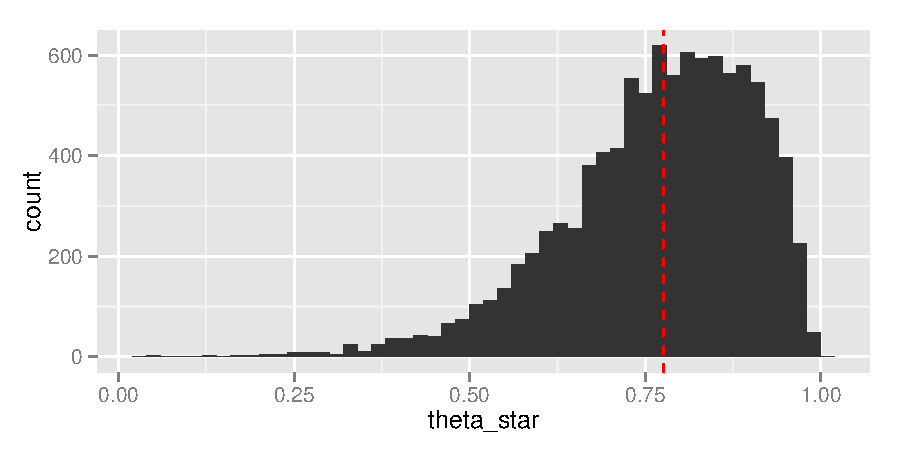
\includegraphics[width=\maxwidth]{figure/chunkname-1} 

\end{knitrout}
When comparing the \texttt{bootstrap} function to the \texttt{boot} function in the package \texttt{boot}, we obtain the same estimate of the standard error. Both run in under 0.2 seconds. The \texttt{boot} function is negligibly faster, but we expect that that time difference may be increased for larger datasets.

\section{Bayesian Bootstrap}
\textcite{Rubin1981} introduced the Bayesian bootstrap (BB) as the natural Bayesian analogue of the bootstrap. Each BB replication generates a posterior probability for each $x_i$, which is centered at $1/n$, but has variability. To obtain a BB replication, first generate a set of weights by drawing $(n-1)$ uniform(0,1) random variates, $u_1, \ldots, u_(n-1)$, ordering them and calculating the gaps $g_t = u_{(t)} - u_{(t-1)}, t=1,\ldots,n$, where $u_{(0)}=0$ and $u_{(n)}=1$. These gaps, $g = (g_1,\ldots,g_n)$ form the weights to attach to the data values in that replication. Considering all the BB replications gives the BB distribution of $X$, and thus of any parameter of this distibution.\\

Our function \texttt{BB} gives a BB distribution. It takes as its inputs a dataset (as a vector, matrix or dataframe), a function for calculating the statistic $\hat{\theta}$ (this function must take two arguments - one for data and one for weights), and $B$, the number of replications required. It returns a list, the first item of which is the standard error of the replicates. The second item is a dataframe with $\theta_1^*,\ldots,\theta_B^*$.

The following code gives the BB distribution when the parameter of interest is the mean. Here the function weighted.mean is in the R base package.
\begin{knitrout}
\definecolor{shadecolor}{rgb}{0.969, 0.969, 0.969}\color{fgcolor}\begin{kframe}
\begin{alltt}
\hlstd{X} \hlkwb{<-} \hlkwd{rnorm}\hlstd{(}\hlnum{100}\hlstd{,} \hlnum{4}\hlstd{,} \hlnum{2}\hlstd{)}
\hlstd{BB_mean} \hlkwb{<-} \hlkwd{BB}\hlstd{(X, weighted.mean,} \hlkwc{B}\hlstd{=}\hlnum{10000}\hlstd{)}
\hlstd{BB_mean}\hlopt{$}\hlstd{se}
\end{alltt}
\begin{verbatim}
## [1] 0.1955357
\end{verbatim}
\end{kframe}
\end{knitrout}

%qplot(T_boot, data=BB_mean$replicates, geom="histogram", binwidth=0.05) + xlab("theta_star")

It may be necessary to define your own function for the statistic of interest that can take weights as an argument. By way of example, we show the BB equivalent of the correlation example from the previous section. The function \texttt{cor} in the R base package cannot take weights; the fuction \texttt{weighted.cor} in our \texttt{Bootstrap} package does.

\begin{knitrout}
\definecolor{shadecolor}{rgb}{0.969, 0.969, 0.969}\color{fgcolor}\begin{kframe}
\begin{alltt}
\hlkwd{set.seed}\hlstd{(}\hlnum{1}\hlstd{)}
\hlstd{BB_law} \hlkwb{<-} \hlkwd{BB}\hlstd{(law_school, weighted.cor,} \hlkwc{B}\hlstd{=}\hlnum{10000}\hlstd{)}
\hlstd{BB_law}\hlopt{$}\hlstd{se}
\end{alltt}
\begin{verbatim}
## [1] 0.1163494
\end{verbatim}
\begin{alltt}
\hlstd{q} \hlkwb{<-} \hlkwd{qplot}\hlstd{(BB_law}\hlopt{$}\hlstd{replicates[,}\hlnum{1}\hlstd{],} \hlkwc{data}\hlstd{=BB_law}\hlopt{$}\hlstd{replicates,} \hlkwc{geom}\hlstd{=}\hlstr{"histogram"}\hlstd{,}
      \hlkwc{binwidth}\hlstd{=}\hlnum{0.02}\hlstd{)} \hlopt{+} \hlkwd{xlab}\hlstd{(}\hlstr{"theta_star"}\hlstd{)}
\hlstd{q} \hlopt{+} \hlkwd{geom_vline}\hlstd{(}\hlkwc{xintercept}\hlstd{=}\hlkwd{cor_df}\hlstd{(law_school),}
               \hlkwc{colour}\hlstd{=}\hlstr{"red"}\hlstd{,} \hlkwc{linetype}\hlstd{=}\hlstr{"dashed"}\hlstd{)}
\end{alltt}
\end{kframe}
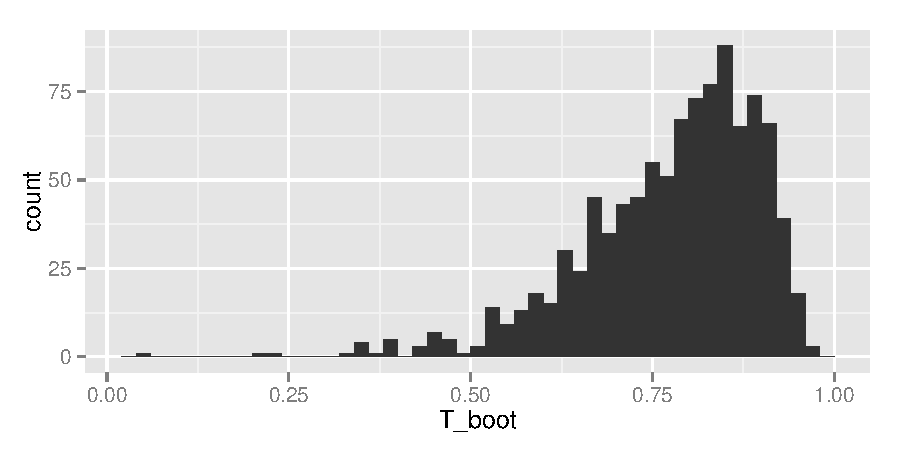
\includegraphics[width=\maxwidth]{figure/unnamed-chunk-3-1} 

\end{knitrout}

In the Bayesian bootstrap, the distribution is tighter around the original sample correlation than in the bootstrap case. In general, \textcite{Rubin1981} points out the inferential similarities between these two methods. As a result, whenever the applicability of the Bayesian bootstrap is called into question, we should also be weary of using the standard bootstrap. Typically, the standard bootstrap is seen as widely applicable, because it is completely non-parametric and does not seem to involve any model assumptions. However, both the bootstrap and Bayesian bootstrap operate under the assumption that all possible values of $X$ have been observed. In any application, the researcher will need to ask themselves whether such an assumption is reasonable. In the Bayesian bootstrap, by using a draw from the uniform Dirichlet distribution for the weights, we are essentially placing a discrete improper prior on the data, which may not be reasonable if the underlying distibution is continuous.

%Furthermore, the BB and the bootstrap make the assumption that there are no relationships between the parameters, which may not be realistic. In such cases, smoothing the parameters may be appropriate. Although there exist models that incorporate smoothing, inference on the parameters will not be the same and neither the bootstrap nor BB can avoid this.

% However, as \textcite{Rubin1981} discusses, the Bayesian bootstrap \emph{does} make model assumptions, namely that SAY MORE...


\section{Bag of Little Bootstraps}
The original bootstrap arose around the time when increases in computing power allowed the development of statistical tools that had previously been too computationally expensive. In recent years, there has been an influx of `big data', alongside the development of parallel computing architectures. \textcite{Kleiner2014} have developed a scalable bootstrap for massive data, known as the Bag of Little Bootstraps (BLB). With massive datasets, the bootstrap's need for recomputation on resamples of the same size as the original dataset is problematic. Rather than obtain bootstrap samples from the whole dataset, the BLB breaks down the process as follows:

\begin{enumerate}
\item Repeatedly ($s$ times) subsample $b(n) < n$ points \emph{without replacement} from the original dataset of size $n$.
\item For each of the $s$ subsamples, do the following:
\begin{enumerate}
\item Repeatedly ($r$ times) resample $n$ point \emph{with replacement} from the subsample.
\item Compute $\hat\theta_n^*$ on each resample.
\item Compute an estimate of $\xi$ based on these $r$ realisations of $\hat\theta_n^*$.
\end{enumerate}
\item We now have one estimate of $\xi$ per subsample. Output their average as the final estimate of $\xi$ for $\hat\theta_n$.
\end{enumerate}

%by taking $s$ subsamples of the original dataset, each of size $b$, where typically $b \ll n$. Each of these subsamples is generated from the original dataset WITHOUT replacement.

\textcite{Kleiner2014} recommend taking $b(n) = n^{\gamma}$, where $\gamma \in [0.5,1]$. This procedure dramatically reduces the size of each resample. For example, if $n$ = 1 million and $\gamma=0.6$, the size of the original dataset may be around 1TB, with a bootstrap resample typically occupying approximately 632GB, and a BLB subsample or resample occupying just 4GB.

The Bootstrap package contains three functions which implement BLB in different cases, \texttt{BLB.1d, BLB.multi} and \texttt{BLB.adapt}. The function \texttt{BLB.1d} implements the simplest version of BLB. It takes as input: a 1-dimensional dataset in a vector; $\gamma$, which controls the value of $b$; a function FUN, which computes the parameter estimate, $\hat\theta_n$. It also takes as arguments $s$ and $r$, which default to 20 and 100 respectively (\textcite{Kleiner2014} demonstates that these values are likely as large as they'll need to be to obtain convergence). The function returns a BLB estimate of $\xi$, which is set as the standard error. When $n=500,000$, the function takes under two minutes to execute (although we compute with a smaller sample here).

\begin{knitrout}
\definecolor{shadecolor}{rgb}{0.969, 0.969, 0.969}\color{fgcolor}\begin{kframe}
\begin{alltt}
\hlstd{X} \hlkwb{<-} \hlkwd{rnorm}\hlstd{(}\hlnum{5000}\hlstd{)}
\hlkwd{BLB.1d}\hlstd{(X, mean,} \hlkwc{gamma}\hlstd{=}\hlnum{0.5}\hlstd{)}
\end{alltt}
\begin{verbatim}
## [1] 0.01355715
\end{verbatim}
\end{kframe}
\end{knitrout}

In their paper, \textcite{Kleiner2014} conduct a simulation study. They generate data from the true underlying distribution, a linear model $Y_i = \tilde X_i^{\top}\textbf{1}_d + \epsilon_i$, with iid $\tilde X_i \sim MVN(0,\mathbb{I}_d)$ and $\epsilon_i \sim N(0,10)$. The estimator $\hat\theta_n$ consists of a linear least squares regression coefficients, with a small $L_2$ penalty of $\lambda=10^{-5}$. To replicate their results, we created the function \texttt{BLB.multi}, which accepts as input an $n \times (d+1)$ dataframe or matrix, where each row is an observation, combining the $d$-dimensional $x$ observation and, in the right-most column, the response, $y$. The tuning parameters for BLB, $\gamma, r$ and $s$, can all be set, as can the tuning parameter $\lambda$ for the penalised regression, and $\alpha$, which controls the width of the confidence intervals. The function returns a list containing the BLB estimate of three quality measures, $\xi^*$: the confidence intervals for each dimension of the estimator, a vector with the width of those intervals, and the standard error of the estimator. As in the paper, we tested the function with $n=20,000$, though we reduced the dimension $d$ from 100 to 10. We chose $\gamma=0.7$, kept $r=100$, and set $s=15$ (which is ample for convergence).

\begin{knitrout}
\definecolor{shadecolor}{rgb}{0.969, 0.969, 0.969}\color{fgcolor}\begin{kframe}
\begin{alltt}
\hlcom{# generate the data}
\hlstd{n}\hlkwb{=}\hlnum{20000}
\hlstd{d}\hlkwb{=}\hlnum{10}
\hlkwd{library}\hlstd{(MASS)}
\hlkwd{set.seed}\hlstd{(}\hlnum{1}\hlstd{)}
\hlstd{X} \hlkwb{<-} \hlkwd{mvrnorm}\hlstd{(n,} \hlkwc{mu}\hlstd{=}\hlkwd{rep}\hlstd{(}\hlnum{0}\hlstd{,d),} \hlkwc{Sigma}\hlstd{=}\hlkwd{diag}\hlstd{(d))}
\hlstd{epsilon} \hlkwb{<-} \hlkwd{rnorm}\hlstd{(n,} \hlkwc{mean}\hlstd{=}\hlnum{0}\hlstd{,} \hlkwc{sd}\hlstd{=}\hlkwd{sqrt}\hlstd{(}\hlnum{10}\hlstd{))}
\hlstd{t_theta} \hlkwb{<-} \hlkwd{as.matrix}\hlstd{(}\hlkwd{rep}\hlstd{(}\hlnum{1}\hlstd{,d))}
\hlstd{Y} \hlkwb{<-} \hlstd{X} \hlopt \hlstd{t_theta} \hlopt{+} \hlstd{epsilon}
\hlstd{data} \hlkwb{<-} \hlkwd{cbind}\hlstd{(X,Y)}

\hlcom{# apply the function and look at the results}
\hlkwd{system.time}\hlstd{(}
  \hlstd{BLB.multi_out} \hlkwb{<-} \hlkwd{BLB.multi}\hlstd{(data,} \hlkwc{gamma}\hlstd{=}\hlnum{0.7}\hlstd{,} \hlkwc{s}\hlstd{=}\hlnum{15}\hlstd{,} \hlkwc{r}\hlstd{=}\hlnum{100}\hlstd{)}
\hlstd{)}
\end{alltt}
\begin{verbatim}
##    user  system elapsed 
##  67.126  14.598  81.759
\end{verbatim}
\begin{alltt}
\hlstd{BLB.multi_out}\hlopt{$}\hlstd{CI_width}
\end{alltt}
\begin{verbatim}
##  [1] 0.08799343 0.08705251 0.08935000 0.08579360 0.08708979 0.09030666
##  [7] 0.08963174 0.08868356 0.08819788 0.08922422
\end{verbatim}
\end{kframe}
\end{knitrout}
As \textcite{Kleiner2014} point out, when $n=20,000$ the true average (across dimensions) marginal confidence interval width for the estimated parameter vector is approximately 0.1, so our function gives the expected results.

\subsection{Adaptive tuning parameter selection}
In \texttt{BLB.multi}, we need to specify values for $s$, the number of subsamples and $r$, the number of bootstrap replicates per subsample. As \textcite{Kleiner2014} discuss, in practice fairly modest values for these tuning parameters often suffice for convergence, though they will vary depending on the value of $\gamma$, as well as on the parameter $\theta$ being estimated and the choice of quality assessment $\xi$. We wish to use the smallest values of $r$ and $s$ which have sufficiently good statistical properties. In order to minimise the computational cost, we can select $r$ and $s$ adaptively. \textcite{Kleiner2014} suggest the following scheme. Suppose we are currenlty processing subsample $j$. We adaptively select $r$ by repeatedly produce resamples, computing the parameter $\theta^{\star}_{n}$ and evaluating $\xi^{\star}_{n}$, until convergence. Convergence is said to have occurred when $\xi^{\star}_{n}$ no longer changes significantly after being updated from a new resample.

The exact measure of convergence is given by the following algorithm: Given a series of realisations of $\xi_n^*$, $ z^{(1)} ,..., z^{(t)}\in \mathbb{R}^{d}$; a window $w \in \mathbb{N}$ ($ w<t $); and a target relative error $\epsilon$,  we keep on producing subsamples until the following condition holds: $\forall j \in [1,w]$,
$ 1/d \sum_{i=1}^{d} | (z_{(i)}^{t-i}-z_{i}^{t} | / |z_{(i)}^{(t)} | \leq \epsilon $.

The same condition can be used for the selection of $s$. Therefore, both parameters can be selected adaptively and in this case $r$ is chosen independently for each subsample. The function \texttt{BLB.adapt} implements BLB with adaptive selection of both $r$ and $s$. It takes data in the same format as \texttt{BLB.multi}, and likewise the parameter of interest is the coefficients of a penalised linear regression. \textcite{Kleiner2014} suggest the values of $w=3$ for the selection of $s$, $w=20$ for the selection of $r$, and $\epsilon=0.05$ for both adaptive procedures. The values of $\gamma, \lambda$ and $\epsilon$ can also be set as arguments, as well as $\alpha$, which controls the width of the confidence intervals. It returns the width of the marginal confidence intervals, along with the final value of $s$, and a vector of the values of $r$ used in each subsample. Here we apply \texttt{BLB.adapt} to the same data as we used above with \texttt{BLB.multi}. Most arguments are set to the default values suggested above.

\begin{knitrout}
\definecolor{shadecolor}{rgb}{0.969, 0.969, 0.969}\color{fgcolor}\begin{kframe}
\begin{alltt}
\hlkwd{set.seed}\hlstd{(}\hlnum{1}\hlstd{)}
\hlkwd{system.time}\hlstd{(}
  \hlstd{BLB.adapt_out} \hlkwb{<-} \hlkwd{BLB.adapt}\hlstd{(data,} \hlkwc{gamma}\hlstd{=}\hlnum{0.7}\hlstd{)}
\hlstd{)}
\end{alltt}
\begin{verbatim}
##    user  system elapsed 
##  17.190   3.715  20.921
\end{verbatim}
\begin{alltt}
\hlstd{BLB.adapt_out}\hlopt{$}\hlstd{s; BLB.adapt_out}\hlopt{$}\hlstd{r}
\end{alltt}
\begin{verbatim}
## [1] 6
## [1] 46 69 60 51 57 76
\end{verbatim}
\begin{alltt}
\hlstd{BLB.adapt_out}\hlopt{$}\hlstd{mean_width}
\end{alltt}
\begin{verbatim}
## [1] 0.09066808
\end{verbatim}
\end{kframe}
\end{knitrout}

We see that both $s$ and $r$ within each subsample are lower than the recommended defaults used in \texttt{BLB.multi}, and consequently \texttt{BLB.adapt} is much faster to run, whilst still returning a value of the mean width of the confidence intervals that is very close to those before. Moreover, the adaptive scheme avoids the problem of having to specify tuning parameters \emph{a priori}, whilst still ensuring good statistical performance. We recommend always using \texttt{BLB.adapt} instead of \texttt{BLB.multi}.

The BLB is well-suited to modern parallel and computing distributed computing environments. It is possible to distribute subsamples to different computer nodes and then parallelize across resamples within each subsample. We have not pursued that line when developing and testing the \texttt{Bootstrap} package.

In our implementation of all three BLB functions, we at some point store all $n$ values in each bootstrap replication. A more effecient implementation would avoid this. Since there are only $b(n)$ possible values in each resample (typically with $b(n) \ll n$), we should only need to know how many times each of these occur in the resample in order to compute $\hat\theta_n^*$. Our implementation is fast enough on the data we have simulated, but we expect that for massive datasets, we would encounter memory problems. The \texttt{BLB.multi} and \texttt{BLB.adapt} functions are also limited to regression problems where the parameter of interest are the coefficients. Future work includes a more generic implementation that can take a wider variety of data types and allow the user to specify a function for estimating any parameter of the underlying distribution.

\printbibliography
\end{document}
